%%%%%%%%%%%%%%%%%%%%%%%%%%%%%%%%%%%%%%%%%%
%%%%%%%%%%%%%                 %%%%%%%%%%%%
%%%%%%%%%%%%%    EXERCISE 1   %%%%%%%%%%%%
%%%%%%%%%%%%%                 %%%%%%%%%%%%
%%%%%%%%%%%%%%%%%%%%%%%%%%%%%%%%%%%%%%%%%%
\begin{exercise}[]{Illustrate the difference between Markov process and Markov decision process.}
  \begin{solution}
  \par{~}
  Markov process is a kind of random process. Its original model markov chain. In the Markov process, given the present state and all past states, the conditional probability distribution of the future state only depends on the current state. In other words, given the present state, it is conditional independent of the past state (that is, the historical path of the process).

  MDP describes the cyclic process in which an Agent takes actions to change its State, obtain Rewards and interact with the Environment. It's an extension of the Markov chain.
  The Markov decision process is a useful tool in the field of dynamic programming and reinforcement learning to solve optimization problems.

  \end{solution}
  \label{ex1}
\end{exercise}


%%%%%%%%%%%%%%%%%%%%%%%%%%%%%%%%%%%%%%%%%%
%%%%%%%%%%%%%                 %%%%%%%%%%%%
%%%%%%%%%%%%%    EXERCISE 2   %%%%%%%%%%%%
%%%%%%%%%%%%%                 %%%%%%%%%%%%
%%%%%%%%%%%%%%%%%%%%%%%%%%%%%%%%%%%%%%%%%%
\begin{exercise}[]{Write out the parameter update equations for TD learning with
    \begin{equation}
        \hat{U}(x,y)=\theta_0 +\theta_1 x + \theta_2 y + \theta_3 \sqrt{(x-x_g)^2+(y-y_g)^2}
    \end{equation}}
  \begin{solution}
  The generalized form of TD Learning with function approximation is given as
  \begin{equation}
    \theta_{i} \leftarrow \theta_{i}+\alpha\left[R(s)+\gamma \hat{U}_{\theta}\left(s^{\prime}\right)-\hat{U}_{\theta}(s)\right] \frac{\partial \hat{U}_{\theta}(s)}{\partial \theta_{i}}
  \end{equation}

  For the approximation function in the problem, the update equations will be
  \begin{equation}
      \begin{aligned}
          \theta_0 & \leftarrow \theta_0 + \alpha\left[R(s)+\gamma \hat{U}_{\theta}\left(s^{\prime}\right)-\hat{U}_{\theta}(s)\right]\\
          \theta_1 & \leftarrow \theta_1 +\alpha\left[R(s)+\gamma \hat{U}_{\theta}\left(s^{\prime}\right)-\hat{U}_{\theta}(s)\right] x\\
          \theta_2 & \leftarrow \theta_2 +\alpha\left[R(s)+\gamma \hat{U}_{\theta}\left(s^{\prime}\right)-\hat{U}_{\theta}(s)\right] y\\
          \theta_3 & \leftarrow \theta_3 +\alpha\left[R(s)+\gamma \hat{U}_{\theta}\left(s^{\prime}\right)-\hat{U}_{\theta}(s)\right] \sqrt{(x-x_g)^2+(y-y_g)^2}\\
      \end{aligned}
  \end{equation}
  \end{solution}
  \label{ex2}
\end{exercise}


%%%%%%%%%%%%%%%%%%%%%%%%%%%%%%%%%%%%%%%%%%
%%%%%%%%%%%%%                 %%%%%%%%%%%%
%%%%%%%%%%%%%    EXERCISE 3   %%%%%%%%%%%%
%%%%%%%%%%%%%                 %%%%%%%%%%%%
%%%%%%%%%%%%%%%%%%%%%%%%%%%%%%%%%%%%%%%%%%
\begin{exercise}[]{阐述强化学习时序差分方法中 on-policy learning 和 off-policy learning 的区别,尝试推导出强化学习 Sarsa 算法的更新公式:
    \begin{equation}
        Q(S,A) = Q(S,A) + \alpha(R + \gamma Q(S',A') - Q(S,A))
    \end{equation}}
  \begin{solution}
    Off-policy learning evaluate and improve a policy that is different from Policy that is used for action selection. A case in point is Q-Learning, where the evaluation phase takes the maximum of the Q-value of all actions that the successor state may take, which is a greedy choice, and is different from the policy we use when choosing the current action (for example, $\epsilon$-greedy).


    On-policy learning evaluate and improve the same policy which is being used to select actions. That means we will try to evaluate and improve the same policy that the agent is already using for action selection. A typical example is SARSA algorithm (for State-Action-Reward-State-Action). Unlike Q-learning, SARSA waits until an action is actually taken and backs up the Q-value for that action. Therefore, we need to replace the $\max_{a'}Q(S',a')$ with the value that is chosen under the same policy $Q(S',a')$. The update equation for SARSA is
    \begin{equation}
        Q(S,A) = Q(S,A) + \alpha(R + \gamma Q(S',A') - Q(S,A))
    \end{equation}
    
    The characteristic of the two learning methods also differs. For off-policy learning like Q-learning, since it may use the best Q-value, it pays no attention to the actual policy being followed, it is more flexible than on-policy learning, in the sense that a Q-learning agent can learn how to behave well even when guided by a random or adversarial exploration policy. 
    
    On the other hand, on-policy learning is more realistic: for example, if the overall policy is even partly controlled by other agents, it is better to learn a Q-function for what will actually happen rather than what the agent would like to happen.
  \end{solution}
  \label{ex3}
\end{exercise}

%%%%%%%%%%%%%%%%%%%%%%%%%%%%%%%%%%%%%%%%%%
%%%%%%%%%%%%%                 %%%%%%%%%%%%
%%%%%%%%%%%%%    EXERCISE 4   %%%%%%%%%%%%
%%%%%%%%%%%%%                 %%%%%%%%%%%%
%%%%%%%%%%%%%%%%%%%%%%%%%%%%%%%%%%%%%%%%%%
\begin{exercise}[]{The MDP bellow has states represented as nodes and transitions as edges between nodes. The rewards for the transitions are indicated by the numbers on the edges. For example,going from state B to state A gives a reward of $10,$ but going from state A to itself gives a reward of $0 .$ Some transitions are not allowed, such as from state A to state $\mathrm{B}$. Transitions are deterministic (if there is an edge between two states, the agent can choose to go from one to the other and will reach the other state with probability 1).

    \begin{figure}[ht]
        \centering
        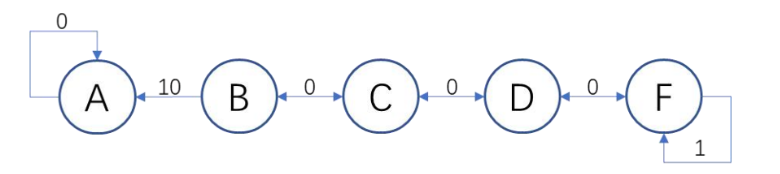
\includegraphics[width = 14cm]{img/ex2.png}
        \caption{Exercise 4}
    \end{figure} 

    1) For this part only, suppose that the max horizon length is $15 .$ Write down the optimal action at each step if the discount factor is $\gamma=1$.

    2) Now suppose that the horizon is infinite. For each state, does the optimal action depend on $\gamma$? If so, for each state, write an equation that would let you determine the value for $\gamma$ at which the optimal action changes.}
  \begin{solution}
  \par{~}
  \begin{enumerate}
      \item {
      \begin{itemize}
          \item A: Go to A
          \item B: Go to C
          \item C: Go to D
          \item D: Go to F
          \item F: Go to F
      \end{itemize}}
      \item {
          W.l.o.g, consider the states except A since A has only one action to take and is trivially independent of $\gamma$. For other nodes, yes.
          
          Stepping from B to A and get reward 10, or stepping to F and iterate forever, getting the reward of $\frac{1}{1-\gamma}$ are the only two ways to achieve maximum rewards.

          \begin{itemize}
              \item For B, $R_1 = 10\gamma$, $R_2 = \frac{\gamma^4}{1-\gamma}$, The optimal action changes at $\gamma^3 + 10 \gamma -10 =0$
              \item For C, $R_1 = 10\gamma^2$, $R_2 = \frac{\gamma^3}{1-\gamma}$, The optimal action changes at $11\gamma - 10 = 0$
              \item For D, $R_1 = 10\gamma^3$, $R_2 = \frac{\gamma^2}{1-\gamma}$, The optimal action changes at $10\gamma^2 - 10\gamma + 1 = 0$
              \item For F, $R_1 = 10\gamma^4$, $R_2 = \frac{\gamma}{1-\gamma}$, The optimal action changes at $10\gamma^4 - 10\gamma^3 + 1 = 0$
          \end{itemize}


      }
  \end{enumerate}
  \end{solution}
  \label{ex4}
\end{exercise}